\section{Zadanie 6}

\subsection{Charakterystyka algorytmu interpolacji trygonometrycznej}

Algorytm interpolacji trygonometrycznej pozwala na aproksymację funkcji okresowych za pomocą wielomianów trygonometrycznych. Złożoność tego algorytmu wynosi \( O(n \cdot m) \), gdzie \( n \) to liczba punktów interpolacyjnych (\( n = 2m \)), a \( m \) jest liczbą współczynników w wielomianie. W szczególności algorytm korzysta z okresowych wartości funkcji w równomiernie rozłożonych węzłach, co pozwala na wyznaczenie współczynników aproksymacji trygonometrycznej. 

W ramach eksperymentu zbadano, jak zmienia się błąd interpolacji w zależności od liczby punktów \( m \) oraz jak dobrze algorytm odtwarza wybrane funkcje (ciągłe i nieciągłe). Wyniki zaprezentowano na wykresach. Ustawienia jak w zadaniu 3/4.


\subsection{Wyniki i wnioski}

\begin{center}
% Wykres błędów dla funkcji
\textbf{Wyniki dla funkcji \( \sin(x) + \cos(x) \):}  
Minimalny błąd: \( 2.22e-16 \)  
Osiągnięty dla \( m = 3 \)  
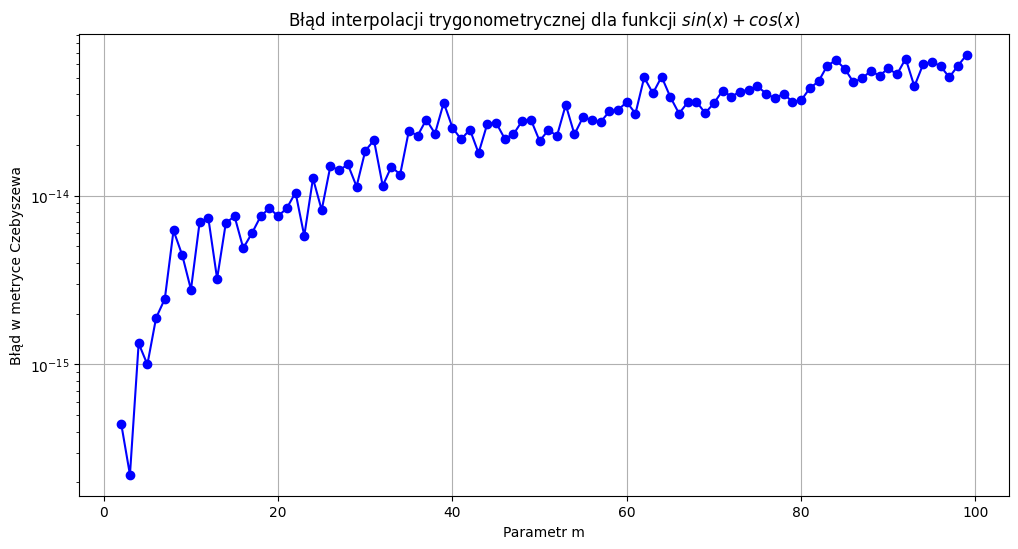
\includegraphics[width=0.8\textwidth]{wykresy/zadanie 5/tryg_blad.png}
\end{center}

\begin{minipage}{0.49\textwidth}
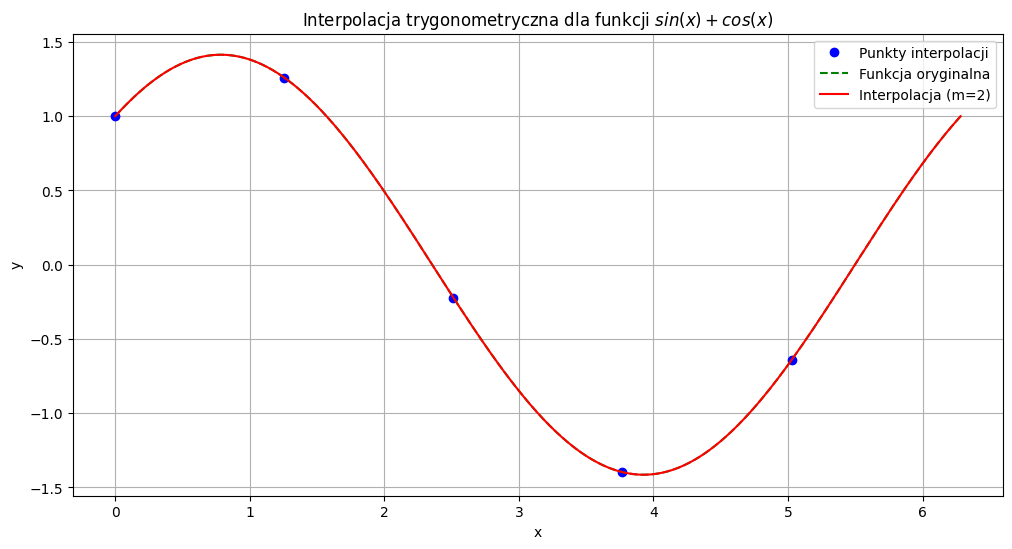
\includegraphics[width=\textwidth]{wykresy/zadanie 5/tryg_2.png}
\end{minipage}
\begin{minipage}{0.49\textwidth}
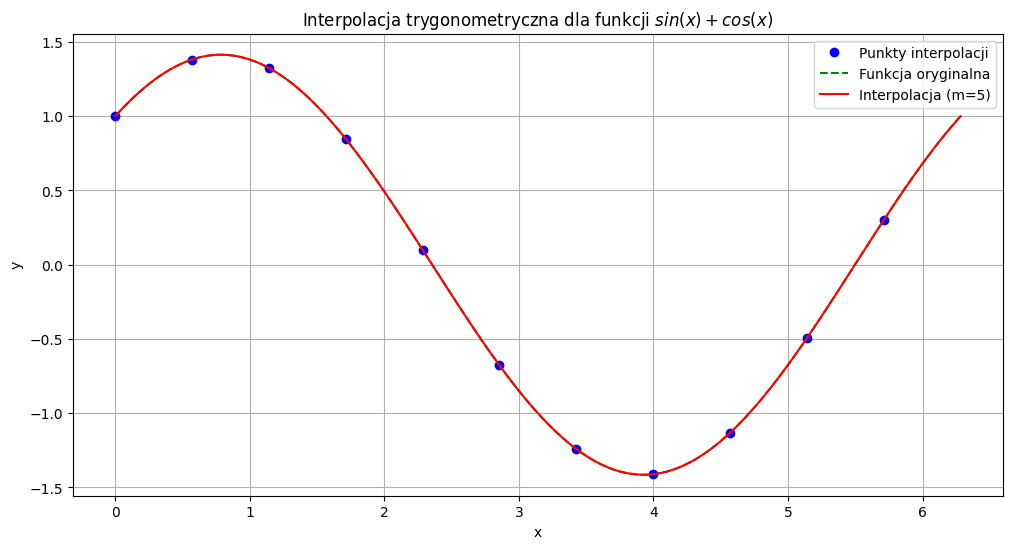
\includegraphics[width=\textwidth]{wykresy/zadanie 5/tryg_5.png}
\end{minipage}

\begin{minipage}{0.49\textwidth}
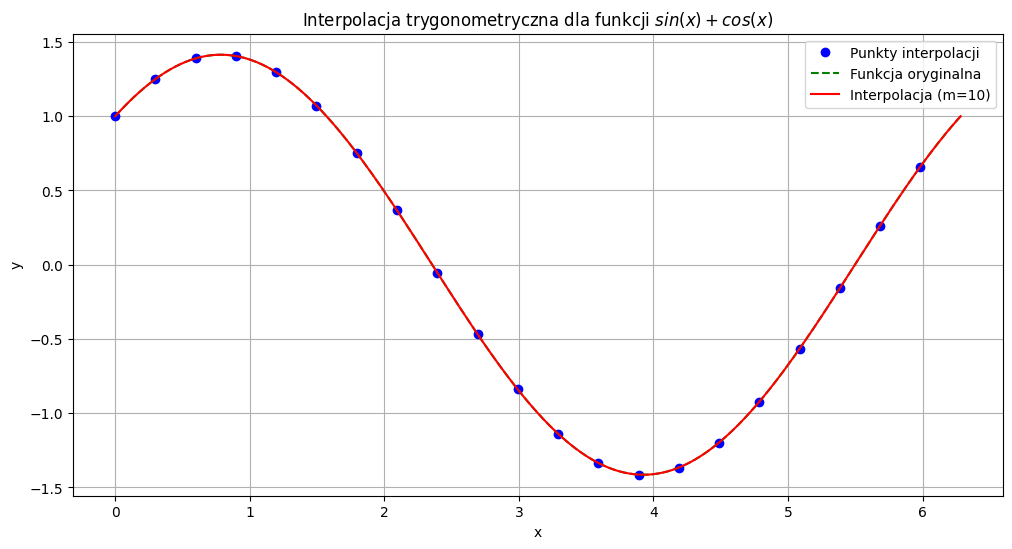
\includegraphics[width=\textwidth]{wykresy/zadanie 5/tryg_10.png}
\end{minipage}
\begin{minipage}{0.49\textwidth}
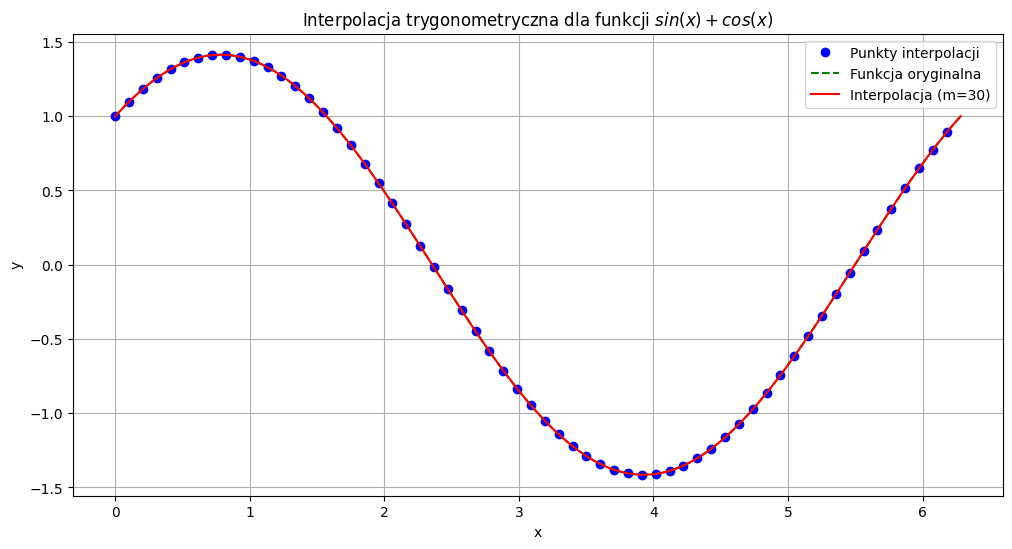
\includegraphics[width=\textwidth]{wykresy/zadanie 5/tryg_30.png}
\end{minipage}

\begin{center}
\textbf{Wyniki dla funkcji \( \frac{1}{1+x^2} \):}  
Minimalny błąd: \( 9.75e-01 \)  
Osiągnięty dla \( m = 89 \)  
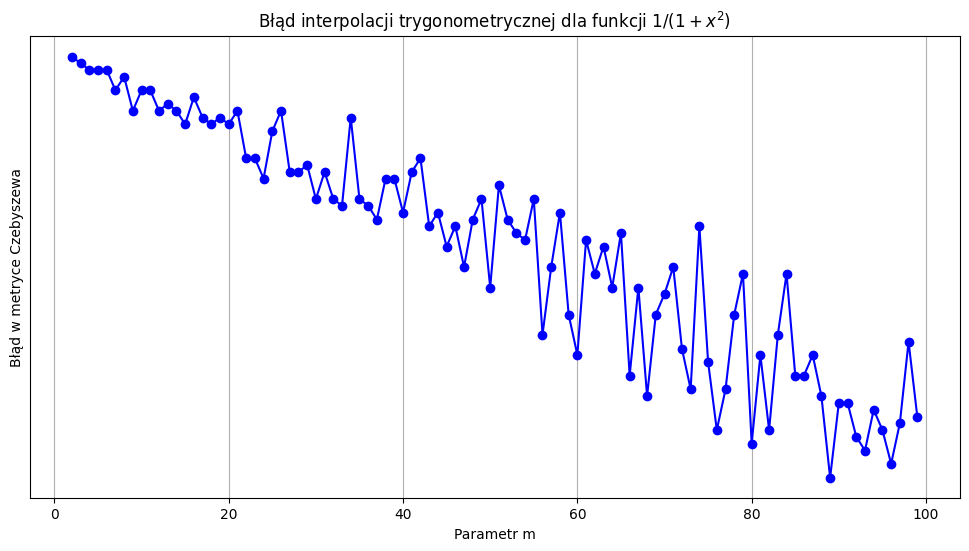
\includegraphics[width=0.8\textwidth]{wykresy/zadanie 5/wym_blad.png}
\end{center}

\begin{minipage}{0.49\textwidth}
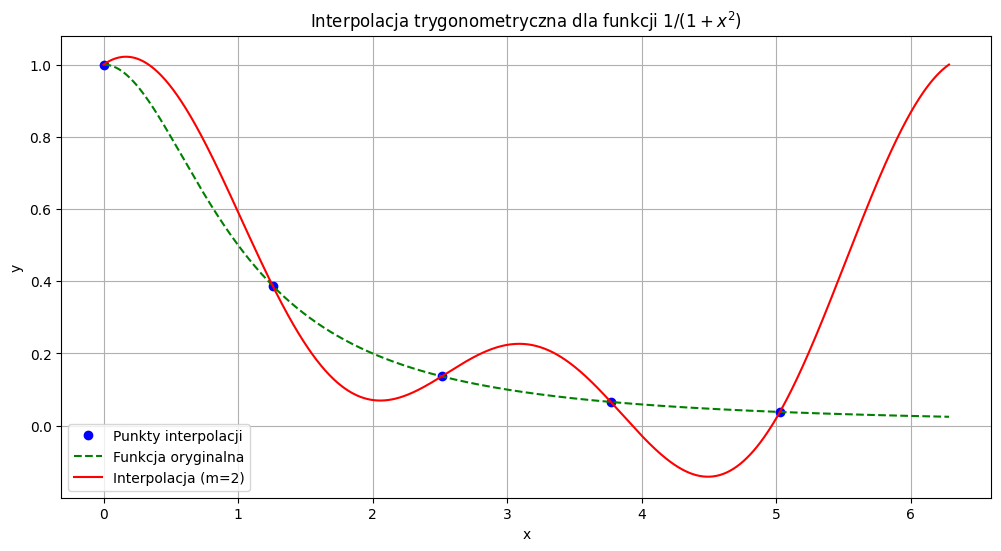
\includegraphics[width=\textwidth]{wykresy/zadanie 5/wym_2.png}
\end{minipage}
\begin{minipage}{0.49\textwidth}
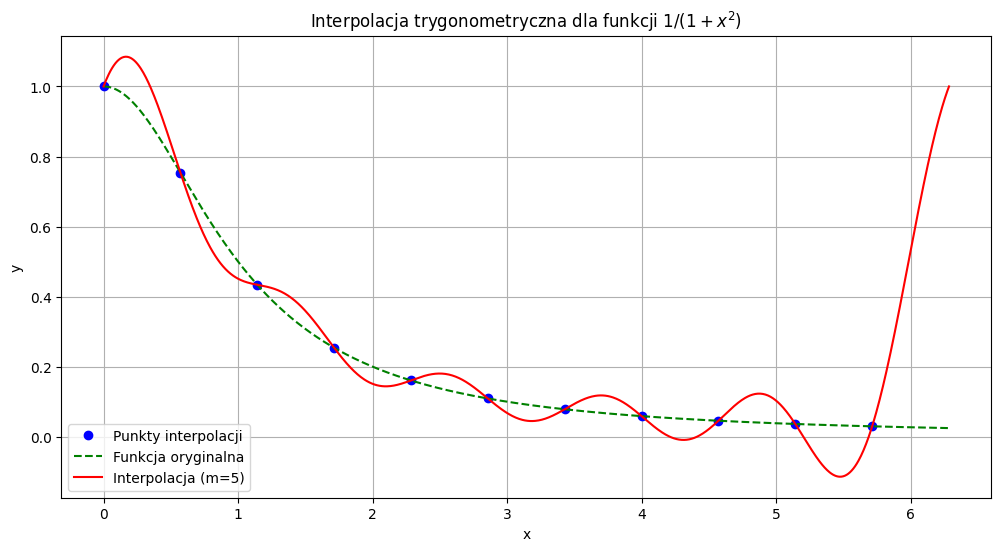
\includegraphics[width=\textwidth]{wykresy/zadanie 5/wym_5.png}
\end{minipage}

\begin{minipage}{0.49\textwidth}
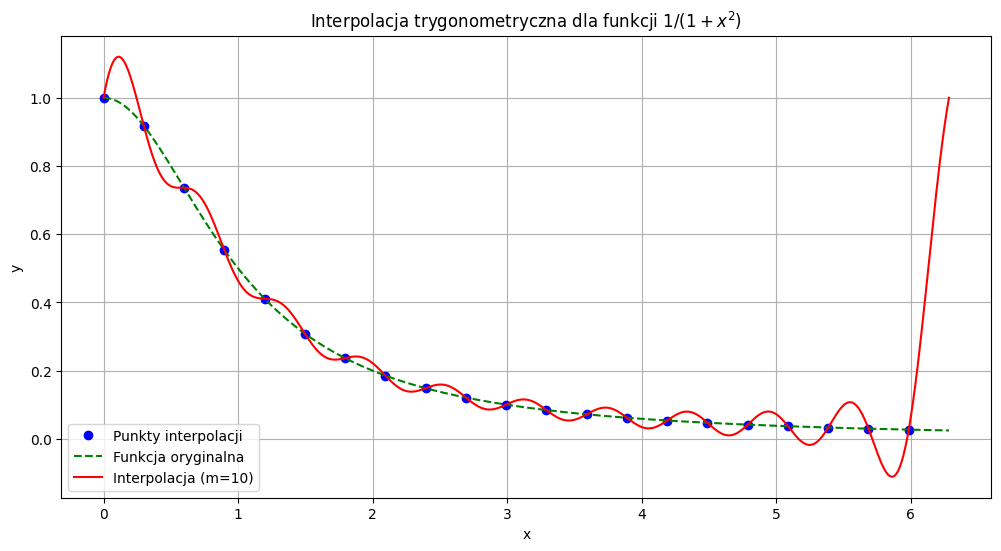
\includegraphics[width=\textwidth]{wykresy/zadanie 5/wym_10.png}
\end{minipage}
\begin{minipage}{0.49\textwidth}
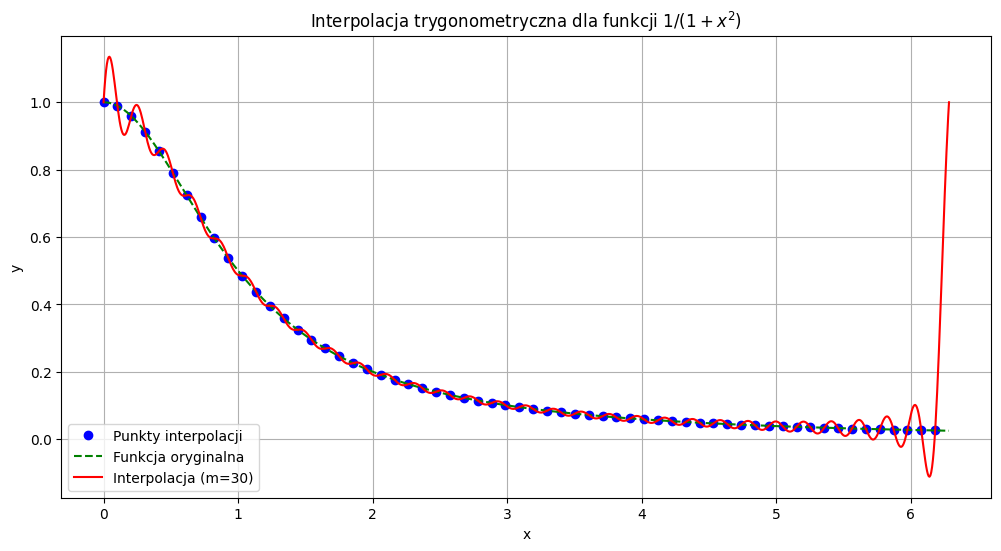
\includegraphics[width=\textwidth]{wykresy/zadanie 5/wym_30.png}
\end{minipage}

\begin{center}
% Wykres błędów dla funkcji podłoga
\textbf{Wyniki dla funkcji podłoga:}  
Minimalny błąd: \( 6.00e+00 \)  
Osiągnięty dla \( m = 99 \)  
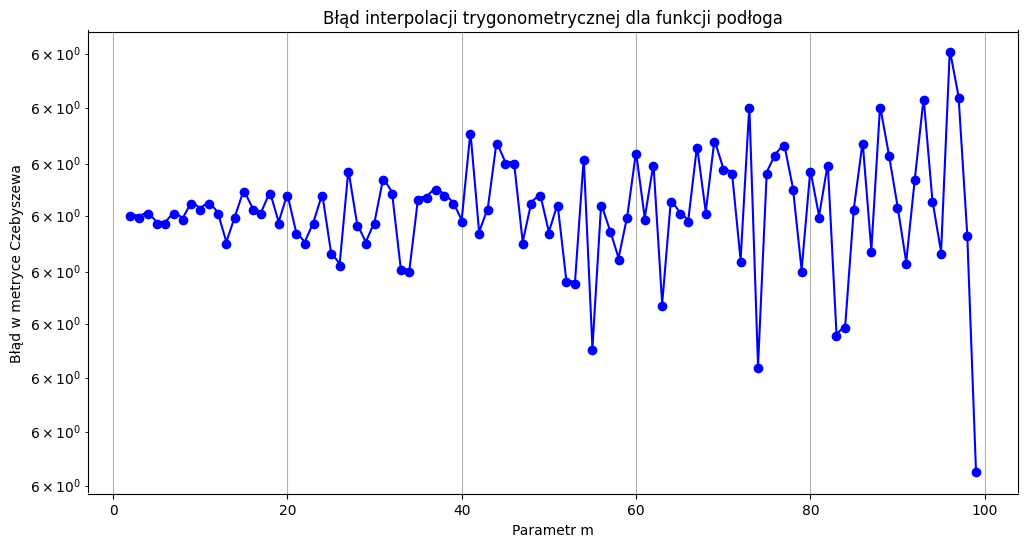
\includegraphics[width=0.8\textwidth]{wykresy/zadanie 5/floor_blad.png}
\end{center}

\begin{minipage}{0.49\textwidth}
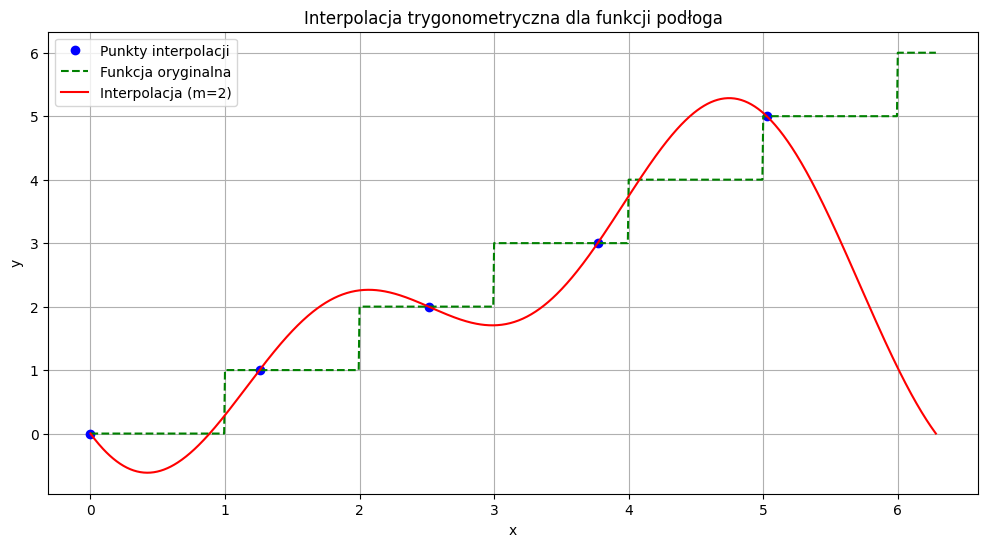
\includegraphics[width=\textwidth]{wykresy/zadanie 5/floor_2.png}
\end{minipage}
\begin{minipage}{0.49\textwidth}
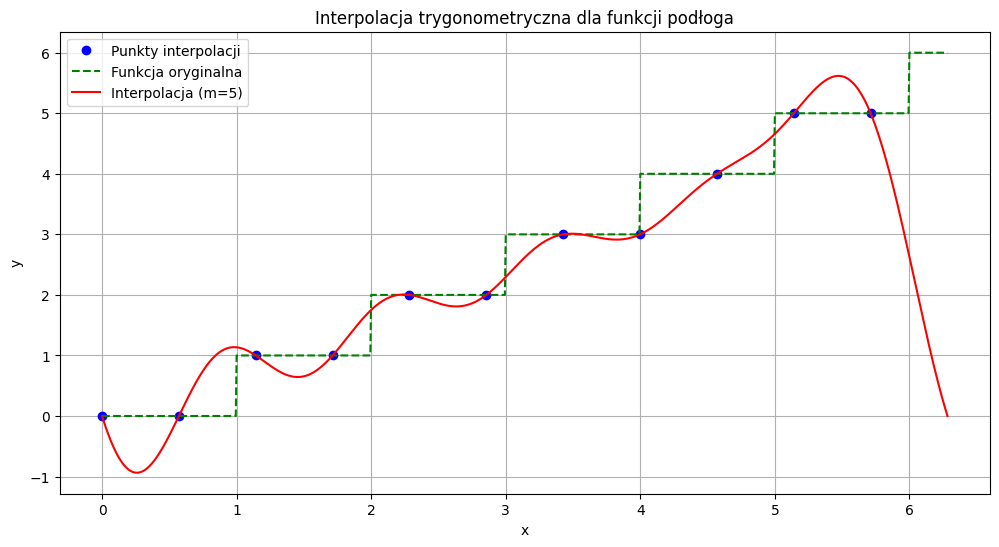
\includegraphics[width=\textwidth]{wykresy/zadanie 5/floor_5.png}
\end{minipage}

\begin{minipage}{0.49\textwidth}
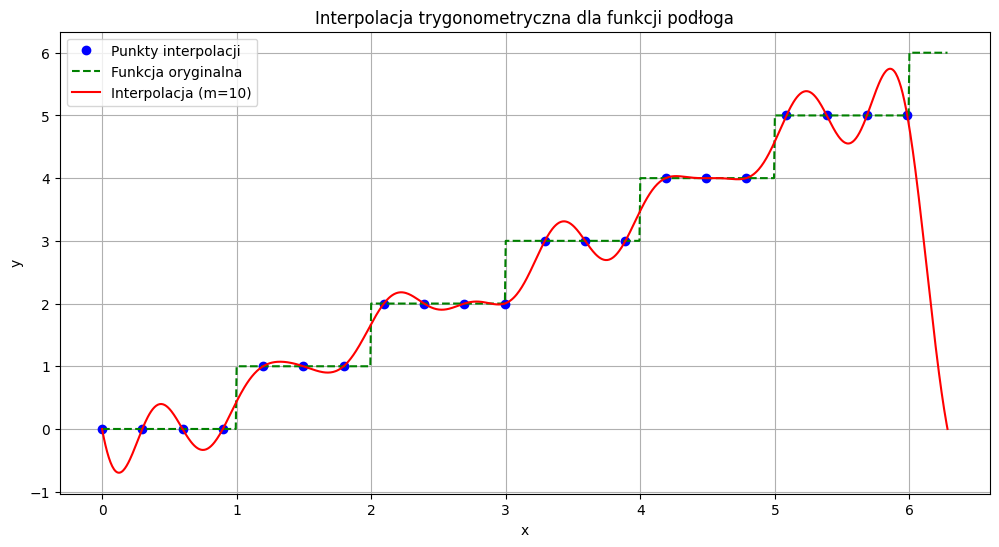
\includegraphics[width=\textwidth]{wykresy/zadanie 5/floor_10.png}
\end{minipage}
\begin{minipage}{0.49\textwidth}
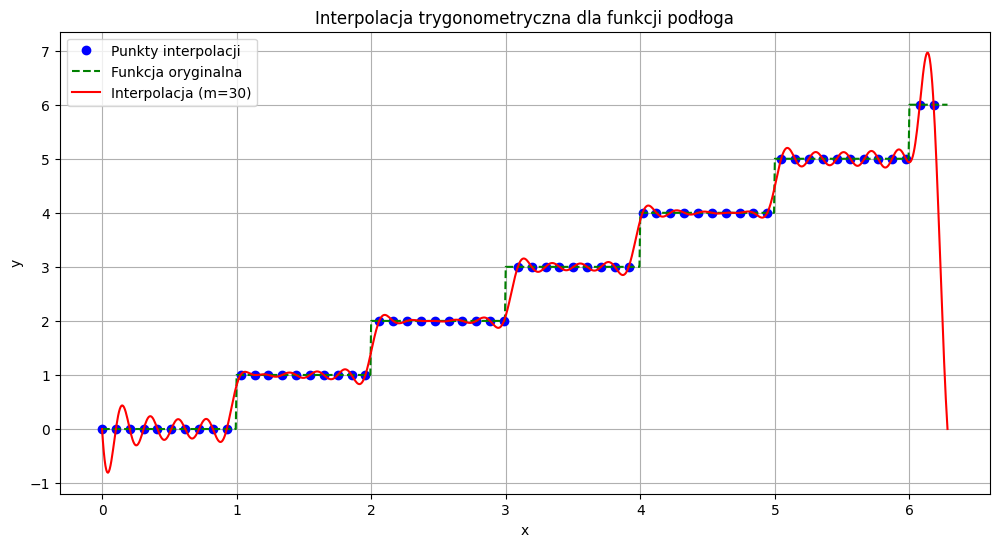
\includegraphics[width=\textwidth]{wykresy/zadanie 5/floor_30.png}
\end{minipage}

\textbf{Wnioski:}
\begin{itemize}
    \item \textbf{Dokładność:} Algorytm interpolacji trygonometrycznej charakteryzuje się bardzo małymi błędami dla funkcji okresowych, takich jak \( \sin(x) + \cos(x) \). 
    \item \textbf{Interpolacja funkcji nieciągłych:} Pomimo swojej specyfiki, algorytm pozwala na interpolację funkcji nieciągłych (np. funkcji podłoga), choć błąd w tych przypadkach jest znacznie większy.
    \item \textbf{Odchylenia na końcach:} Wahania na końcu wykresów błędu wynikają z niedoskonałości implementacji, co można skorygować. W teorii, metoda powinna dawać wyniki zgodne z oczekiwaniami.
    \item \textbf{Uniwersalność:} Dzięki możliwości skalowania dziedziny do \( [0, 2\pi] \), metoda ma szerokie zastosowania i może być wykorzystywana do analizy wielu rodzajów funkcji.
\end{itemize}


